\documentclass{beamer}
\usepackage[utf8]{inputenc}
\usepackage{graphicx, epsfig}
\usepackage{amsmath,mathrsfs,amsfonts,amssymb}
\usepackage{floatflt}
\usepackage{epic,ecltree}
\usepackage{mathtext}
\usepackage{fancybox}
\usepackage{fancyhdr}
\usepackage{multirow}
\usepackage{enumerate}
\usepackage{epstopdf}
\usepackage{multicol}
\usepackage{algorithm}
\usepackage[noend]{algorithmic}
\usepackage{tikz}
\usepackage{blindtext}
\usetheme{default}%{Singapore}%{Warsaw}%{Warsaw}%{Darmstadt}
\usecolortheme{default}

\setbeamerfont{title}{size=\Huge}
\setbeamertemplate{footline}[page number]{}

\setbeamertemplate{section in toc}[sections numbered]


\makeatletter
\newcommand\HUGE{\@setfontsize\Huge{35}{40}}
\makeatother    

\setbeamerfont{title}{size=\HUGE}
\beamertemplatenavigationsymbolsempty

% latin bold lower
\newcommand{\ba}{\mathbf{a}} 
\newcommand{\bc}{\mathbf{c}} 
\newcommand{\be}{\mathbf{e}} 
\newcommand{\bff}{\mathbf{f}} % \bf - for bold type
\newcommand{\bg}{\mathbf{g}} 
\newcommand{\bh}{\mathbf{h}} 
\newcommand{\bp}{\mathbf{p}} 
\newcommand{\bq}{\mathbf{q}} 
\newcommand{\bt}{\mathbf{t}} 
\newcommand{\bs}{\mathbf{s}} 
\newcommand{\bu}{\mathbf{u}} 
\newcommand{\bv}{\mathbf{v}} 
\newcommand{\bw}{\mathbf{w}} 
\newcommand{\bx}{\mathbf{x}} 
\newcommand{\by}{\mathbf{y}} 
\newcommand{\bz}{\mathbf{z}} 

% latin bold upper
\newcommand{\bA}{\mathbf{A}} 
\newcommand{\bB}{\mathbf{B}} 
\newcommand{\bC}{\mathbf{C}} 
\newcommand{\bG}{\mathbf{G}} 
\newcommand{\bI}{\mathbf{I}} 
\newcommand{\bJ}{\mathbf{J}} 
\newcommand{\bL}{\mathbf{L}} 
\newcommand{\bM}{\mathbf{M}} 
\newcommand{\bP}{\mathbf{P}}
\newcommand{\bQ}{\mathbf{Q}} 
\newcommand{\bR}{\mathbf{R}} 
\newcommand{\bT}{\mathbf{T}} 
\newcommand{\bU}{\mathbf{U}} 
\newcommand{\bV}{\mathbf{V}} 
\newcommand{\bW}{\mathbf{W}} 
\newcommand{\bX}{\mathbf{X}} 
\newcommand{\bY}{\mathbf{Y}} 
\newcommand{\bZ}{\mathbf{Z}} 

% latin cal upper
\newcommand{\cF}{\mathcal{F}} 
\newcommand{\cG}{\mathcal{G}} 
\newcommand{\cI}{\mathcal{I}} 
\newcommand{\cL}{\mathcal{L}} 
\newcommand{\cM}{\mathcal{M}} 
\newcommand{\cN}{\mathcal{N}} 
\newcommand{\cP}{\mathcal{P}} 
\newcommand{\cS}{\mathcal{S}} 
\newcommand{\cT}{\mathcal{T}} 
\newcommand{\cW}{\mathcal{W}} 
\newcommand{\cX}{\mathcal{X}} 
\newcommand{\cZ}{\mathcal{Z}} 

% latin bb upper
\newcommand{\bbE}{\mathbb{E}} 
\newcommand{\bbI}{\mathbb{I}} 
\newcommand{\bbP}{\mathbb{P}} 
\newcommand{\bbR}{\mathbb{R}} 

% greek bold lower
\newcommand{\bepsilon}{\boldsymbol{\epsilon}} 
\newcommand{\btheta}{\boldsymbol{\theta}} 
\newcommand{\blambda}{\boldsymbol{\lambda}} 
\newcommand{\bpi}{\boldsymbol{\pi}} 
\newcommand{\bmu}{\boldsymbol{\mu}} 
\newcommand{\bsigma}{\boldsymbol{\sigma}} 
\newcommand{\bphi}{\boldsymbol{\phi}} 

% greek bold upper
\newcommand{\bSigma}{\boldsymbol{\Sigma}} 

\DeclareMathOperator*{\argmin}{arg\,min}
\DeclareMathOperator*{\argmax}{arg\,max}
\newcommand{\createdgmtitle}[1]{\title[\hbox to 56mm{Deep Generative Models  \hfill\insertframenumber\,/\,\inserttotalframenumber}]
	{\vspace{1cm} \\ \textbf{Deep Generative Models} \\ {\Huge Lecture #1}}
	\author{Roman Isachenko}
		\institute{
\includegraphics[width=0.7cm]{../utils/aimasterslogo} \LARGE{AI Masters}}
	\date{2025, Spring}
}

\usepackage{tikz}
\usetikzlibrary{arrows,shapes,positioning,shadows,trees}

\newcommand\myfootnote[1]{%
  \tikz[remember picture,overlay]
  \draw (current page.south west) +(1in + \oddsidemargin,0.5em)
  node[anchor=south west,inner sep=0pt]{\parbox{\textwidth}{%
      \rlap{\rule{10em}{0.4pt}}\raggedright\scriptsize \textit{#1}}};}

\newcommand\myfootnotewithlink[2]{%
  \tikz[remember picture,overlay]
  \draw (current page.south west) +(1in + \oddsidemargin,0.5em)
  node[anchor=south west,inner sep=0pt]{\parbox{\textwidth}{%
      \rlap{\rule{10em}{0.4pt}}\raggedright\scriptsize\href{#1}{\textit{#2}}}};}
      
\AtBeginSection[]
      {
      	\begin{frame}{Outline}
      		\tableofcontents[currentsection]
      	\end{frame}
      }
      \AtBeginSubsection[]{
      	\begin{frame}{Outline}
      		\tableofcontents[currentsection,currentsubsection]
      	\end{frame}
}
\createdgmtitle{7}
\usepackage{tikz}

\usetikzlibrary{arrows,shapes,positioning,shadows,trees}
%--------------------------------------------------------------------------------
\begin{document}
%--------------------------------------------------------------------------------
\begin{frame}[noframenumbering,plain]
%\thispagestyle{empty}
\titlepage
\end{frame}
%=======
\begin{frame}{Recap of previous lecture}
	\begin{block}{Likelihood-free learning}
		\begin{itemize}
			\item Likelihood is not a perfect metric for generative model.
			\item Likelihood could be intractable.
		\end{itemize}
	\end{block}
	Imagine we have two sets of samples 
	\begin{itemize}
		\item $\{\bx_i\}_{i=1}^{n_1} \sim \pi(\bx)$ -- real samples;
		\item $\{\bx_i\}_{i=1}^{n_2} \sim p(\bx | \btheta)$ -- generated (or fake) samples.
	\end{itemize}
	\[
		p(y = 1 | \bx) = P\bigl(\{\bx \sim \pi(\bx)\}\bigr); \quad p(y = 0 | \bx) = P\bigl(\{\bx \sim p(\bx | \btheta)\}\bigr)
	\]
	\vspace{-0.5cm}
	\begin{block}{Assumption}
		Generative distribution $p(\bx | \btheta)$ equals to the true distribution $\pi(\bx)$ if we can not distinguish them using discriminative model $p(y | \bx)$. \\
		It means that $p(y = 1 | \bx) = 0.5$ for each sample $\bx$.
	\end{block}
	\begin{itemize}
		\item \textbf{Generator:} generative model $\bx = \bG(\bz)$, which makes generated sample more realistic.
		\item \textbf{Discriminator:} a classifier $D(\bx) \in [0, 1]$, which distinguishes real samples from generated samples.
	\end{itemize}
\end{frame}
%=======
\begin{frame}{Recap of previous lecture}
	\begin{block}{GAN optimality theorem}
		The minimax game 
		\[
		\min_{G} \max_D \Bigl[ \underbrace{\bbE_{\pi(\bx)} \log D(\bx) + \bbE_{p(\bz)} \log (1 - D(\bG(\bz)))}_{V(G, D)} \Bigr]
		\]
		has the global optimum $\pi(\bx) = p(\bx | \btheta)$, in this case $D^*(\bx) = 0.5$.
	\end{block}
	\vspace{-0.3cm} 
	\[
		\min_{G} V(G, D^*) = \min_{G} \left[ 2 JSD(\pi || p) - \log 4 \right] = -\log 4, \quad \pi(\bx) = p(\bx | \btheta).
	\]
	If the generator could be \textbf{any} function and the discriminator is \textbf{optimal} at every step, then the generator is \textbf{guaranteed to converge} to the data distribution.
	 \myfootnotewithlink{https://arxiv.org/abs/1406.2661}{Goodfellow I. J. et al. Generative Adversarial Networks, 2014}
\end{frame}
%=======
\begin{frame}{Recap of previous lecture}
	\begin{itemize}
		\item Generator updates are made in parameter space, discriminator is not optimal at every step.
		\item Generator and discriminator loss keeps oscillating during GAN training.
	\end{itemize}
	\begin{block}{Objective}
		\vspace{-0.5cm}
		\[
		\min_{\btheta} \max_{\bphi} \left[ \bbE_{\pi(\bx)} \log D_{\bphi}(\bx) + \bbE_{p(\bz)} \log (1 - D_{\bphi}(\bG_{\btheta}(\bz))) \right]
		\]
		\vspace{-0.5cm}
	\end{block}
	\begin{figure}
		\centering
		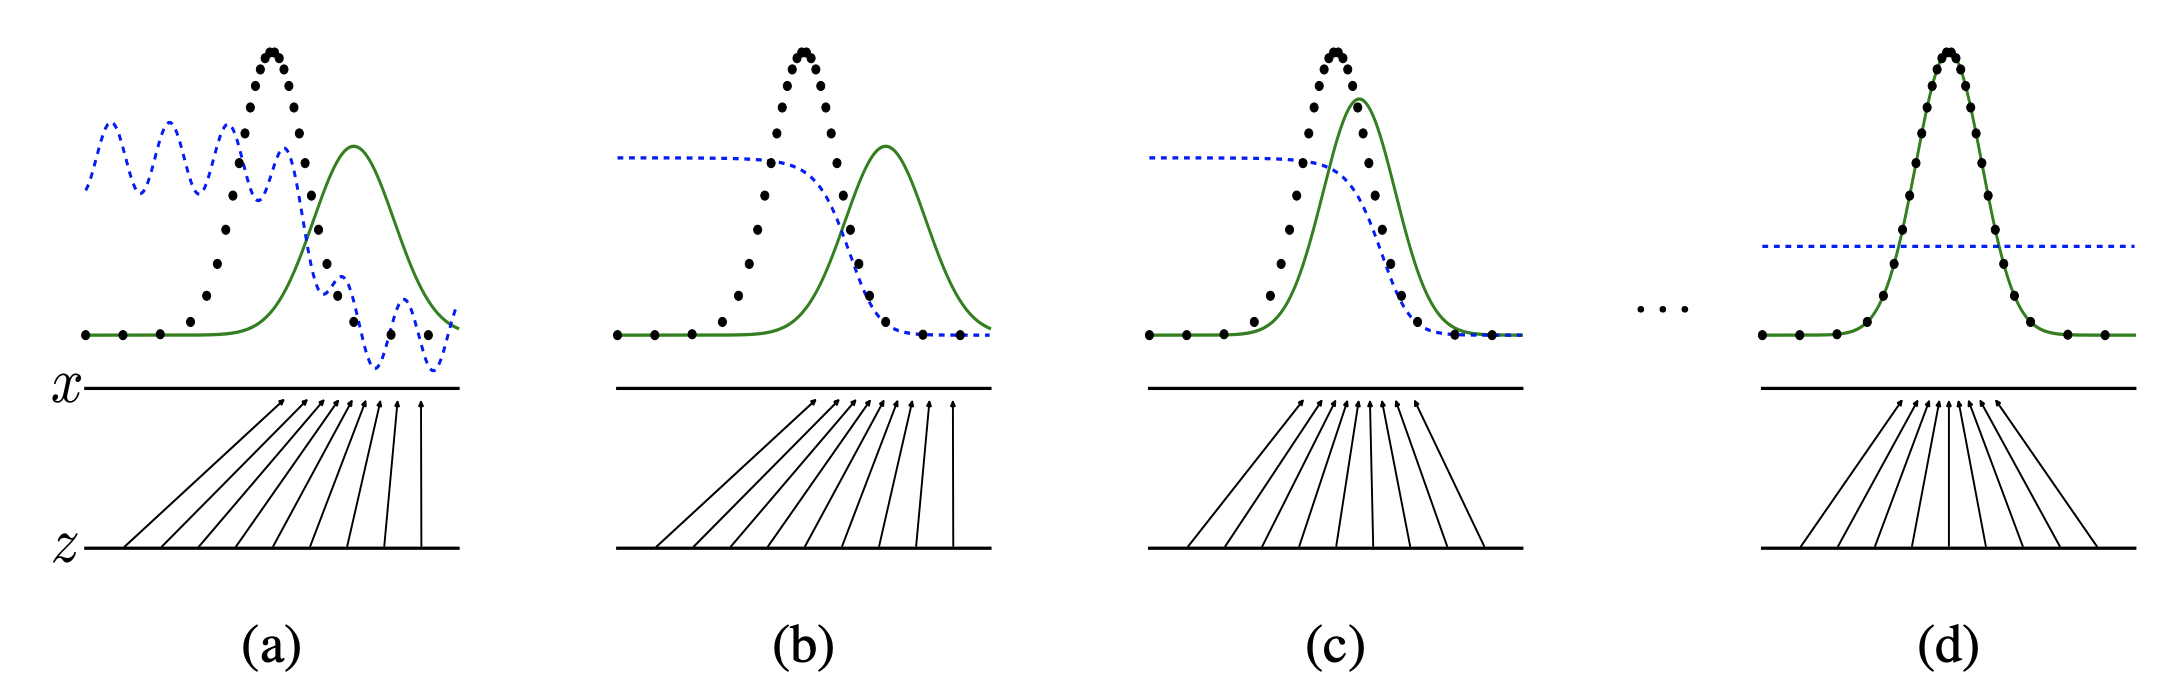
\includegraphics[width=1.0\linewidth]{figs/gan_1}
	\end{figure}
	\myfootnotewithlink{https://arxiv.org/abs/1406.2661}{Goodfellow I. J. et al. Generative Adversarial Networks, 2014}
\end{frame}
%=======
\begin{frame}{Recap of previous lecture}
	\begin{block}{Main problems of standard GAN}
		\begin{itemize}
			\item Vanishing gradients (solution: non-saturating GAN);
			\item Mode collapse (caused by Jensen-Shannon divergence).
		\end{itemize}
	\end{block}
	\begin{block}{Standard GAN}
		\vspace{-0.2cm}
		\[
		\min_{\btheta} \max_{\bphi} \left[ \bbE_{\pi(\bx)} \log D_{\bphi}(\bx) + \bbE_{p(\bz)} \log (1 - D_{\bphi}(\bG_{\btheta}(\bz))) \right]
		\]
		\vspace{-0.4cm}
	\end{block}
	\vspace{-0.1cm}
	\begin{block}{Informal theoretical results}
		The real images distribution $\pi(\bx)$ and the generated images distribution $p(\bx | \btheta)$ are low-dimensional and have disjoint supports. In this case
		\vspace{-0.3cm}
		\[
		KL(\pi || p) = KL(p || \pi) = \infty, \quad JSD(\pi || p) = \log 2.
		\]
	\end{block}
	\myfootnote{\href{https://arxiv.org/abs/1406.2661}{Goodfellow I. J. et al. Generative Adversarial Networks, 2014} \\
		\href{https://arxiv.org/abs/1701.04862}{Arjovsky M., Bottou L. Towards Principled Methods for Training Generative Adversarial Networks, 2017}}
\end{frame}
%=======
\begin{frame}{Recap of previous lecture}
	\begin{figure}
		\centering
		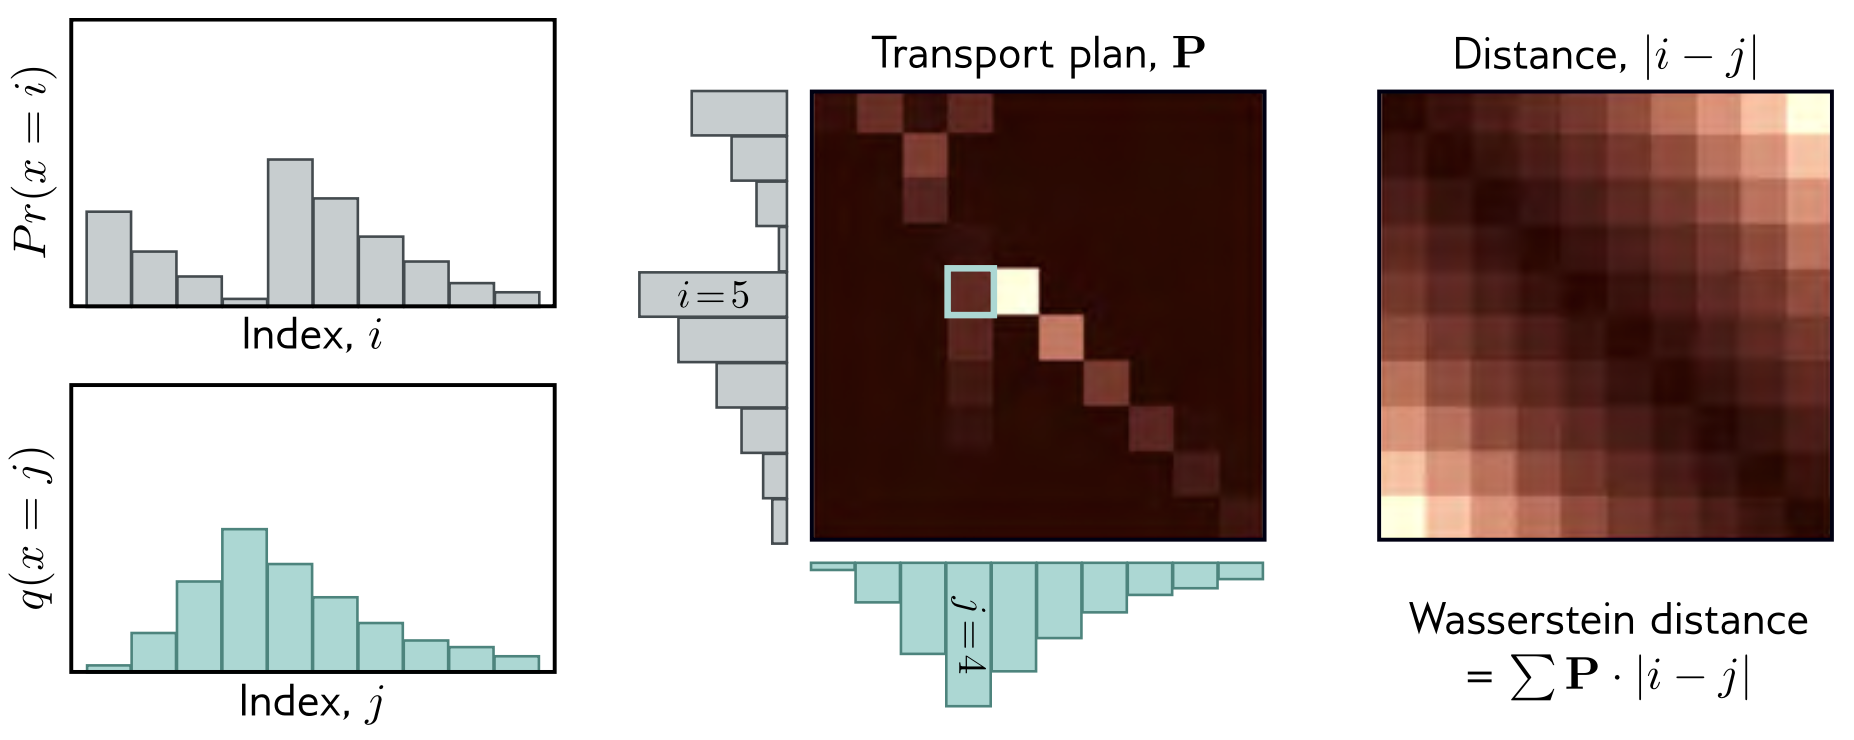
\includegraphics[width=0.8\linewidth]{figs/discrete_wasserstein}
	\end{figure}
	\vspace{-0.3cm}
	\begin{block}{Wasserstein distance}
		\vspace{-0.7cm}
		\[
		W(\pi, p) = \inf_{\gamma \in \Gamma(\pi, p)} \bbE_{(\bx, \by) \sim \gamma} \| \bx - \by \| =  \inf_{\gamma \in \Gamma(\pi, p)} \int \| \bx - \by \| \gamma (\bx, \by) d \bx d \by
		\]
		\vspace{-0.5cm}
		\begin{itemize}
			\item $\gamma(\bx, \by)$ -- transportation plan (the amount of "dirt" that should be transported from point $\bx$ to point $\by$).
			\item $\Gamma(\pi, p)$ -- the set of all joint distributions $\gamma (\bx, \by)$ with marginals $\pi$ and $p$ ($\int \gamma(\bx, \by) d \bx = p(\by)$, $\int \gamma(\bx, \by) d \by = \pi(\bx)$).
			\item $\gamma(\bx, \by)$ -- the amount, $\|\bx - \by \|$-- the distance.
		\end{itemize}
	\end{block}
	\myfootnotewithlink{https://udlbook.github.io/udlbook/}{Simon J.D. Prince. Understanding Deep Learning, 2023}
\end{frame}
%=======
\begin{frame}{Recap of previous lecture}
	\begin{block}{Theorem (Kantorovich-Rubinstein duality)}
		\vspace{-0.2cm}
		\[
		W(\pi || p) = \frac{1}{K} \max_{\| f \|_L \leq K} \left[ \bbE_{\pi(\bx)} f(\bx)  - \bbE_{p(\bx)} f(\bx)\right],
		\]
		where $\| f \|_L \leq K$ are $K-$Lipschitz continuous functions.
	\end{block}
	\begin{block}{WGAN objective}
		\vspace{-0.3cm}
		\[
		\min_{\btheta} {\color{violet}W(\pi || p)} = \min_{\btheta} {\color{violet}\max_{\bphi \in \boldsymbol{\Phi}} \left[ \bbE_{\pi(\bx)} f_{\bphi}(\bx)  - \bbE_{p(\bz)} f_{\bphi}(\bG_{\btheta}(\bz))\right]}.
		\]
		\vspace{-0.3cm}
	\end{block}
	\begin{itemize}
		\item Function~$f$ in WGAN is usually called $\textit{critic}$.
		\item If parameters $\bphi$ lie in a compact set $\boldsymbol{\Phi} \in [-c, c]^d$ then $f(\bx, \bphi)$ will be $K$-Lipschitz continuous function. 
	\end{itemize}
	\begin{multline*}
		K \cdot W(\pi || p) = \max_{\| f \|_L \leq K} \left[ \bbE_{\pi(\bx)} f(\bx)  - \bbE_{p(\bx)} f(\bx)\right] \geq \\  \geq \max_{\bphi \in \boldsymbol{\Phi}} \left[ \bbE_{\pi(\bx)} f_{\bphi}(\bx)  - \bbE_{p(\bx)} f_{\bphi}(\bx)\right]
	\end{multline*}
	\myfootnotewithlink{https://arxiv.org/abs/1701.07875}{Arjovsky M., Chintala S., Bottou L. Wasserstein GAN, 2017}
\end{frame}
%=======
\begin{frame}{Outline}
	\tableofcontents
\end{frame}
%=======
\section{Evaluation of likelihood-free models}
%=======
\begin{frame}{Evaluation of likelihood-free models}
	\begin{block}{Likelihood-based models}
		\begin{itemize}
			\item \textbf{train part:} fit the model.
			\item \textbf{validation part:} tune the hyperparameters.
			\item \textbf{test part:} evaluate generalization by reporting the likelihood.
		\end{itemize}
	\end{block}
	Not all models have tractable likelihood \\ (VAE: compare ELBO values; GAN: \textbf{???}).
	\begin{block}{What do we want from samples?}
		\begin{itemize}
			\item Sharpness
			\begin{figure}
				\centering
				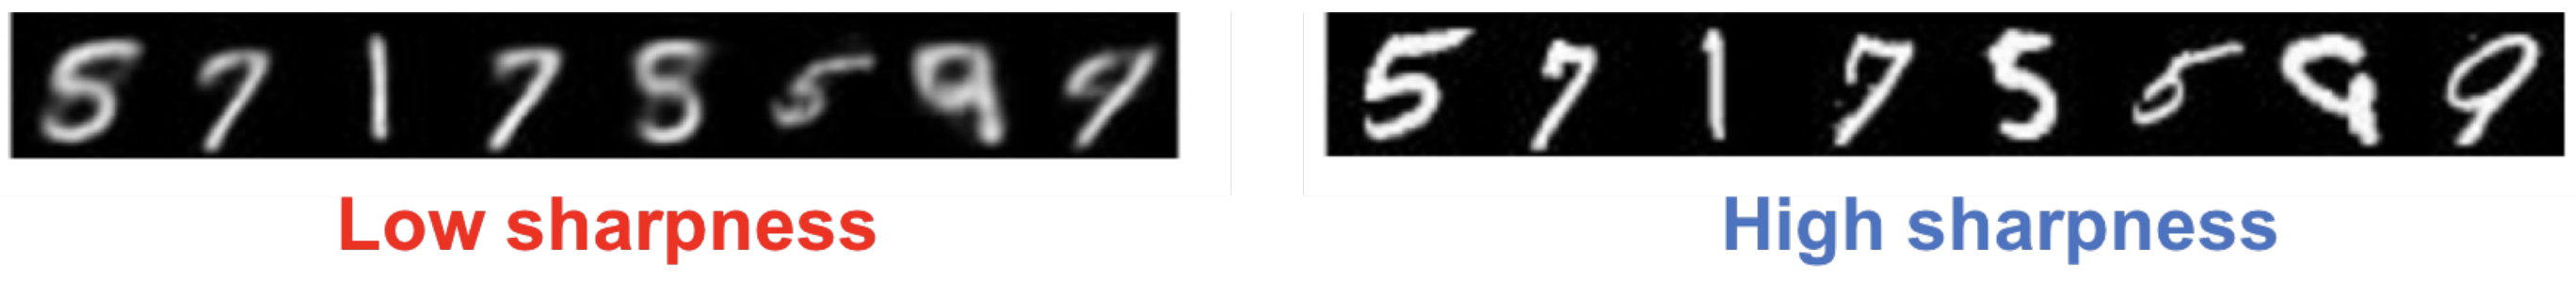
\includegraphics[width=0.9\linewidth]{figs/sharpness}
			\end{figure}
			\item Diversity
			\begin{figure}
				\centering
				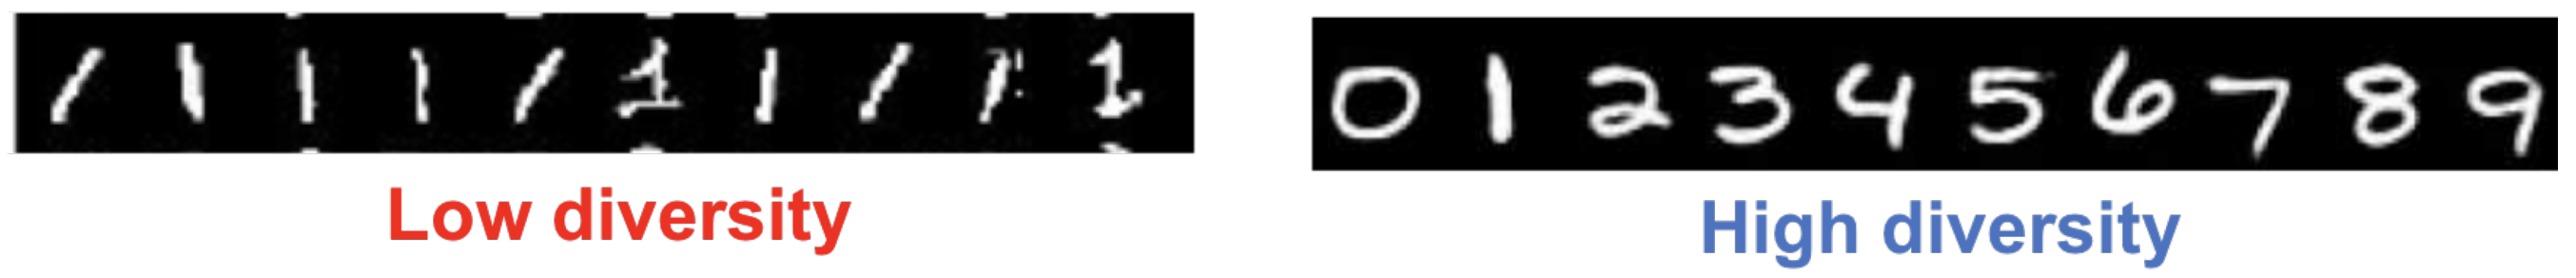
\includegraphics[width=0.9\linewidth]{figs/diversity}
			\end{figure}
		\end{itemize}
	\end{block}
	\myfootnotewithlink{https://deepgenerativemodels.github.io}{image credit: https://deepgenerativemodels.github.io}
\end{frame}
%=======
\subsection{Frechet Inception Distance (FID)}
%=======
\begin{frame}{Wasserstein metric}
	\vspace{-0.2cm}
	\[
		W_s(\pi, p) = \inf_{\gamma \in \Gamma(\pi, p)} \left(\bbE_{(\bx, \by) \sim \gamma} \| \bx - \by \|^s\right)^{1/s}
	\]
	\vspace{-0.3cm}
	\begin{block}{Wassestein GAN (optimal transport)}
		\vspace{-0.5cm}
		\[
			W(\pi, p) = \inf_{\gamma \in \Gamma(\pi, p)} \bbE_{(\bx, \by) \sim \gamma} \| \bx - \by \| =  \inf_{\gamma\in {\Gamma(\pi, p)}} \int { \| \bx - \by \|} {\gamma (\bx, \by)} d \bx d \by
		\]
		\vspace{-0.5cm}
	\end{block}
	\begin{block}{Theorem}
		If $\pi(\bx) = \cN(\bmu_\pi, \bSigma_\pi)$, $p(\by) = \cN(\bmu_p, \bSigma_p)$, then
		\vspace{-0.2cm}
		\[
		W_2^2(\pi, p) = \| \bmu_{\pi} - \bmu_{p}\|^2 + \text{tr} \left[ \bSigma_{\pi} + \bSigma_p - 2 \left(\bSigma_{\pi}^{1/2} \bSigma_p \bSigma_{\pi}^{1/2} \right)^{1/2} \right]
		\]
		\vspace{-0.7cm}
	\end{block}
	\begin{block}{Frechet Inception Distance}
		\vspace{-0.3cm}
		\[
			\text{FID} (\pi, p) =  W_2^2(\pi, p)
		\]
		\vspace{-0.6cm}
	\end{block}
	\myfootnotewithlink{https://arxiv.org/abs/1706.08500}{Heusel M. et al. GANs Trained by a Two Time-Scale Update Rule Converge to a Local Nash Equilibrium, 2017}
\end{frame}
%=======
\begin{frame}{Frechet Inception Distance (FID)}
	\vspace{-0.3cm}
	\[
		\text{FID} (\pi, p) = \| \bmu_{\pi} - \bmu_{p}\|^2 + \text{tr} \left[ \bSigma_{\pi} + \bSigma_p - 2 \left(\bSigma_{\pi}^{1/2} \bSigma_p \bSigma_{\pi}^{1/2} \right)^{1/2} \right]
	\]
	\vspace{-0.5cm}
	\begin{itemize}
		\item FID is calculated in the latent space $\bz$.
		\item We take pretrained image embedder to get the latent representations $\bz = \bff(\bx)$.
		\item $\bmu_{\pi}$, $\bSigma_{\pi}$ and $\bmu_{p}$, $\bSigma_p$ are the statistics of the latent representations $\bz$ for the samples from $\pi(\bx)$ and $p(\bx | \btheta)$.
	\end{itemize}
	\begin{block}{$FID(p(\bx), \cN(0, \bI))$}
		\begin{figure}
			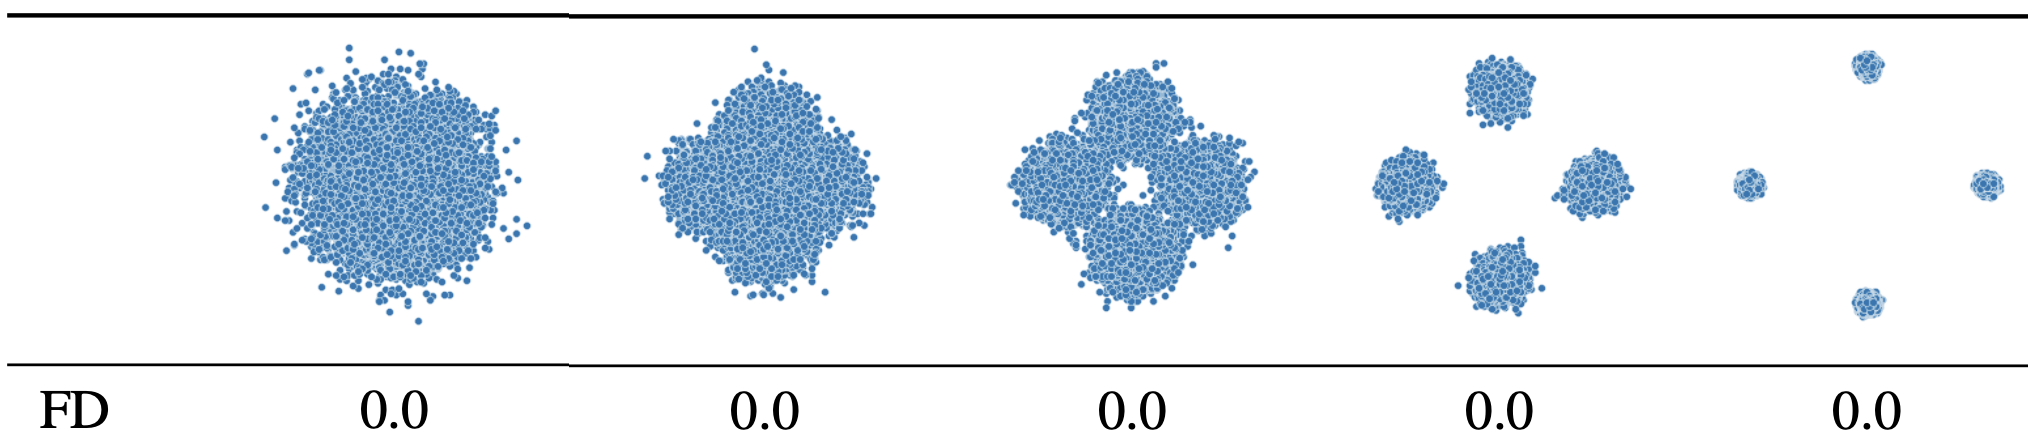
\includegraphics[width=0.95\linewidth]{figs/fid_normal}
		\end{figure}
	\end{block}
	\myfootnotewithlink{https://arxiv.org/abs/2401.09603}{Jayasumana S. et al. Rethinking FID: Towards a Better Evaluation Metric for Image Generation, 2024}
\end{frame}
%=======
\begin{frame}{Frechet Inception Distance (FID)}
	\vspace{-0.4cm}
	\[
	\text{FID} (\pi, p) =  \| \bmu_{\pi} - \bmu_{p}\|^2 + \text{tr} \left[ \bSigma_{\pi} + \bSigma_p - 2 \left(\bSigma_{\pi}^{1/2} \bSigma_p \bSigma_{\pi}^{1/2} \right)^{1/2} \right]
	\]
	\vspace{-0.3cm}
	\begin{block}{Drawbacks}
		\begin{itemize}
			\item Dependence on the pretrained classification model.
			\item Usage of the normality assumption.
			\item May not correspond to human evaluation.
		\end{itemize}
	\end{block}
	
	\begin{figure}
		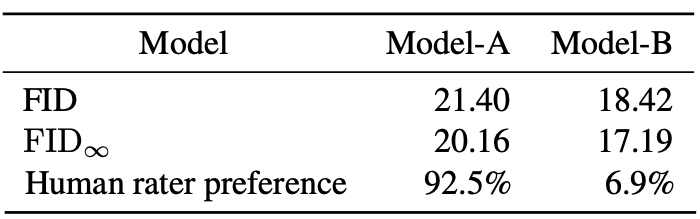
\includegraphics[width=0.7\linewidth]{figs/fid_vs_human_eval}
	\end{figure}
	\myfootnotewithlink{https://arxiv.org/abs/2401.09603}{Jayasumana S. et al. Rethinking FID: Towards a Better Evaluation Metric for Image Generation, 2024}
\end{frame}
%=======
\subsection{Precision-Recall}
%=======
\begin{frame}{Precision-Recall}
	\begin{block}{What do we want from samples}
		\begin{itemize}
			\item \textbf{Sharpness}: generated samples should be of high quality.
			\item \textbf{Diversity}: their variation should match that observed in the training set.
		\end{itemize}
	\end{block}
	\vspace{-0.5cm}
	\begin{figure}
		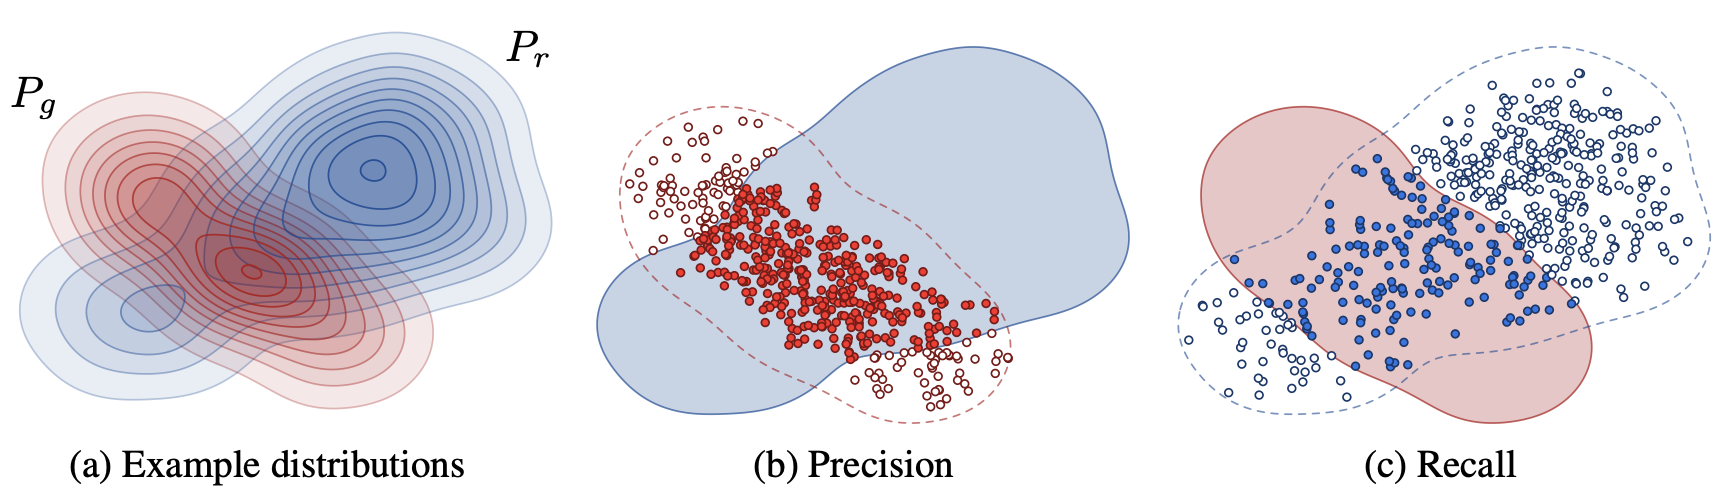
\includegraphics[width=0.95\linewidth]{figs/pr_curve}
	\end{figure}
	\vspace{-0.3cm}
	\begin{itemize}
		\item \textbf{Precision} denotes the fraction of generated images that are realistic.
		\item \textbf{Recall} measures the fraction of the training data manifold covered by the generator.
	\end{itemize}
	\myfootnotewithlink{https://arxiv.org/abs/1904.06991}{Kynkäänniemi T. et al. Improved precision and recall metric for assessing generative models, 2019}
\end{frame}
%=======
\begin{frame}{Precision-Recall}
	\vspace{-0.2cm}
	\begin{itemize}
		\item $\cS_{\pi} = \{\bx_i\}_{i=1}^{n} \sim \pi(\bx)$ -- real samples;
		\item $\cS_{p} = \{\bx_i\}_{i=1}^{n} \sim p(\bx | \btheta)$ -- generated samples.
	\end{itemize}
	Define binary function:
	\vspace{-0.2cm}
	\[
		\mathbb{I}(\bx, \cS) = 
		\begin{cases}
			1, \quad \text{if exists } \bx' \in \cS: \| \bx  - \bx'\|_2 \leq \| \bx' - \text{NN}_k(\bx', \cS)\|_2; \\
			0, \quad \text{otherwise.}
		\end{cases}
	\]
	\vspace{-0.3cm}
	\[
		\text{Precision} (\cS_{\pi}, \cS_{p}) = \frac{1}{n} \sum_{\mathbf{\bx} \in \cS_{p}} \mathbb{I}(\bx, \cS_{\pi}); \,\, \text{Recall} (\cS_{\pi}, \cS_{p}) = \frac{1}{n} \sum_{\bx \in \cS_{\pi}} \mathbb{I}(\bx, \cS_{p}).
	\]
	\vspace{-0.6cm}
	\begin{figure}
		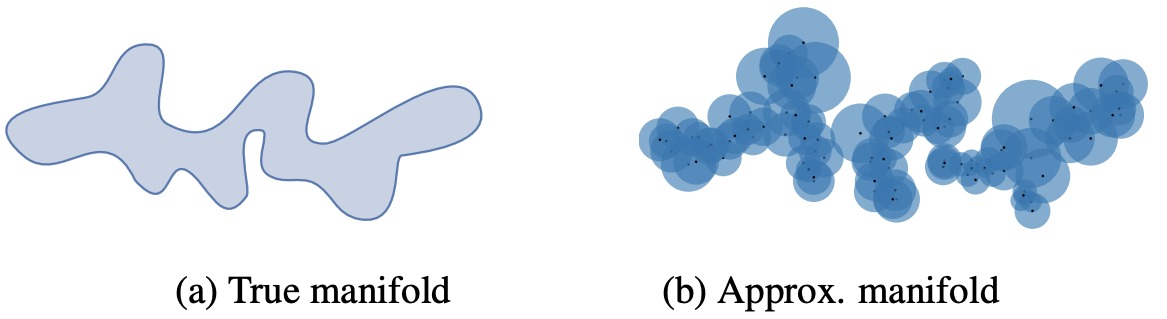
\includegraphics[width=0.75\linewidth]{figs/pr_k_nearest}
	\end{figure}
	Embed the samples using the pretrained network (as for FID).
	\myfootnotewithlink{https://arxiv.org/abs/1904.06991}{Kynkäänniemi T. et al. Improved precision and recall metric for assessing generative models, 2019}
\end{frame}
%=======
\begin{frame}{Precision-Recall}
	\begin{figure}
		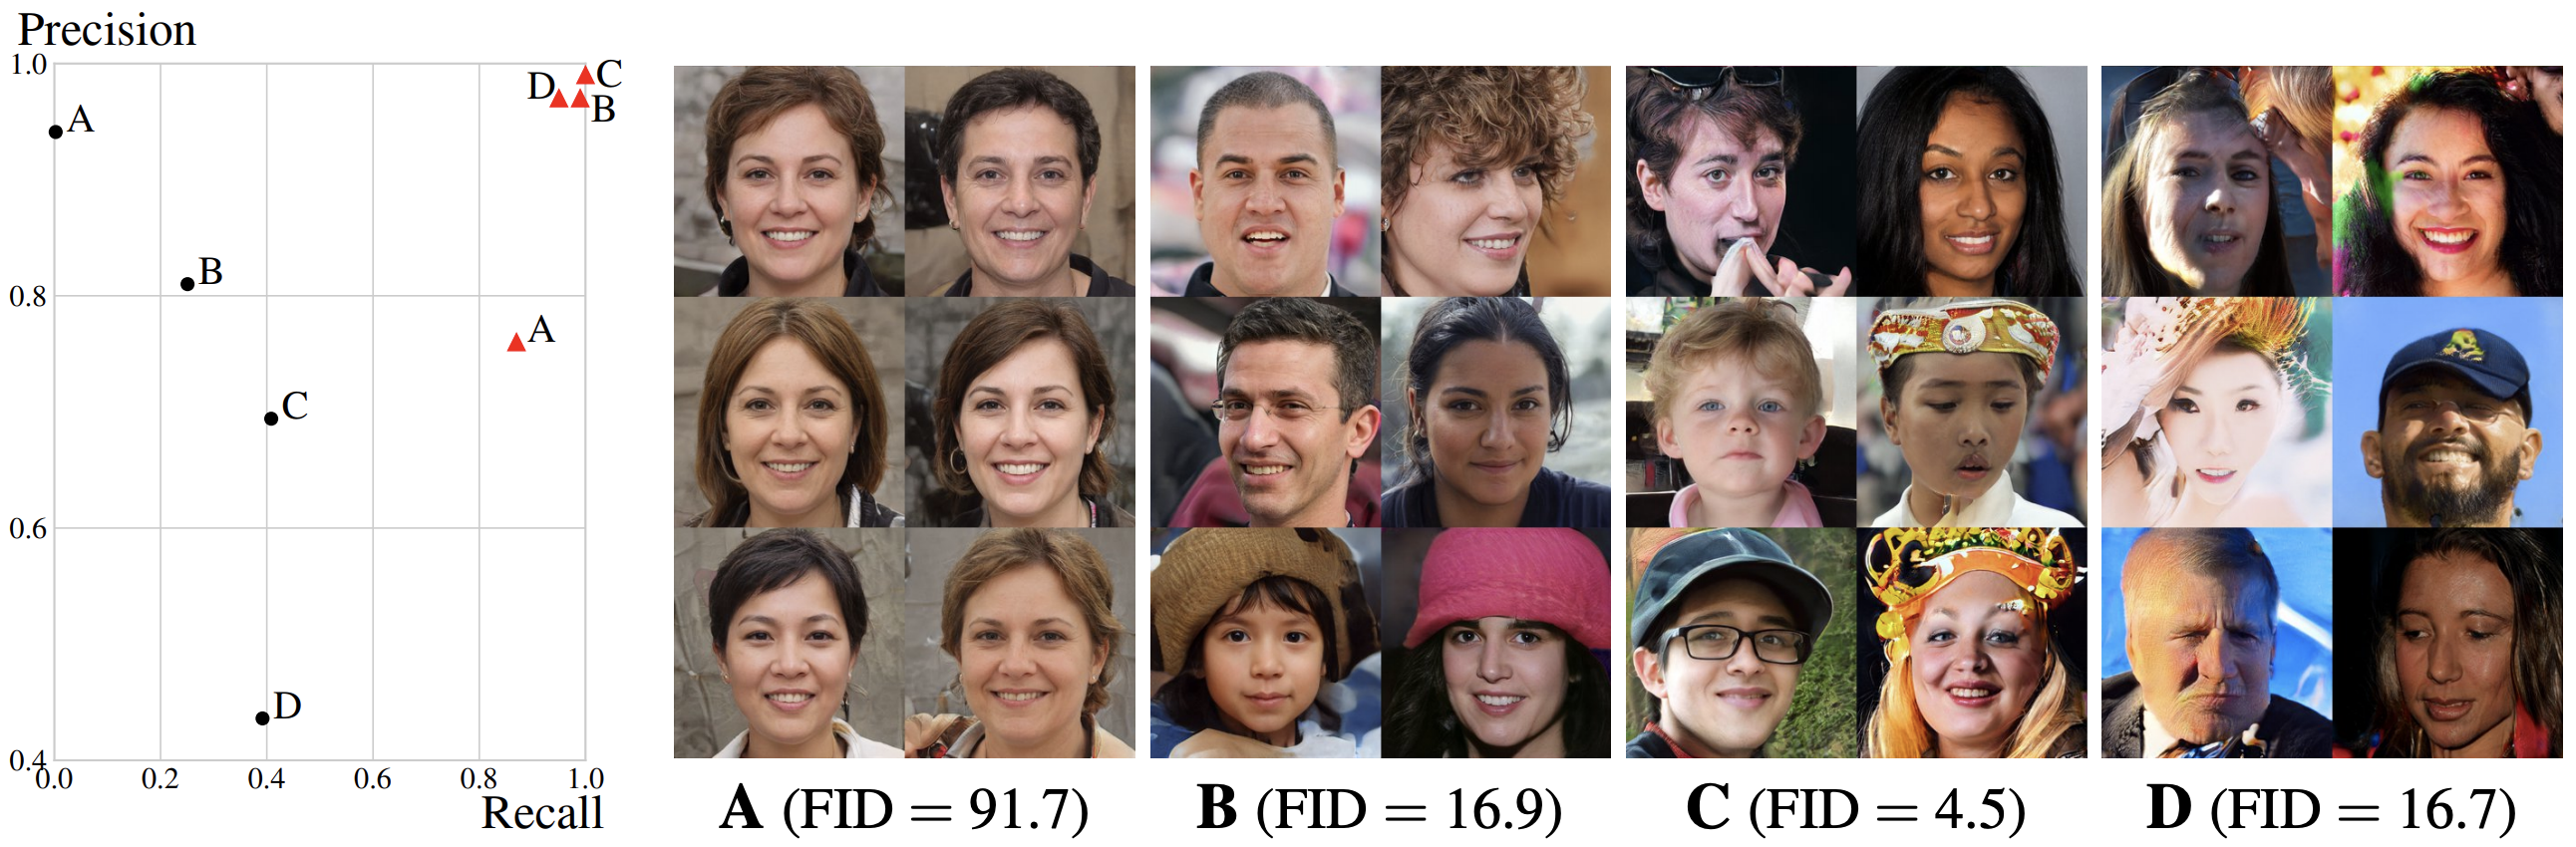
\includegraphics[width=\linewidth]{figs/pr_vs_fid}
	\end{figure}
	\begin{figure}
		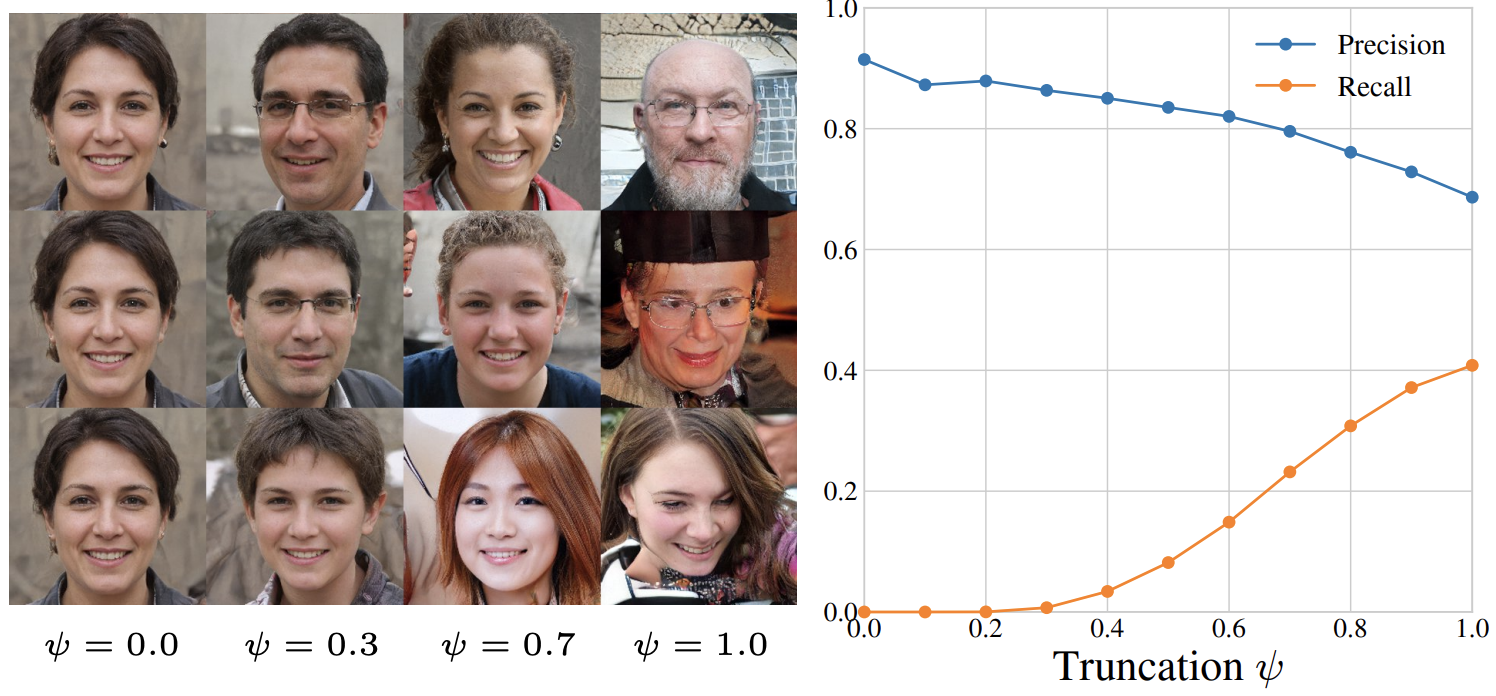
\includegraphics[width=0.75\linewidth]{figs/pr_truncation}
	\end{figure}
	\myfootnotewithlink{https://arxiv.org/abs/1904.06991}{Kynkäänniemi T. et al. Improved precision and recall metric for assessing generative models, 2019}
\end{frame}
%=======
\subsection{CLIP score}
%=======
\begin{frame}{CLIP score}
	\vspace{-0.2cm}
	\begin{minipage}{0.5\linewidth}
		\begin{block}{Unconditional model}
			\begin{figure}
				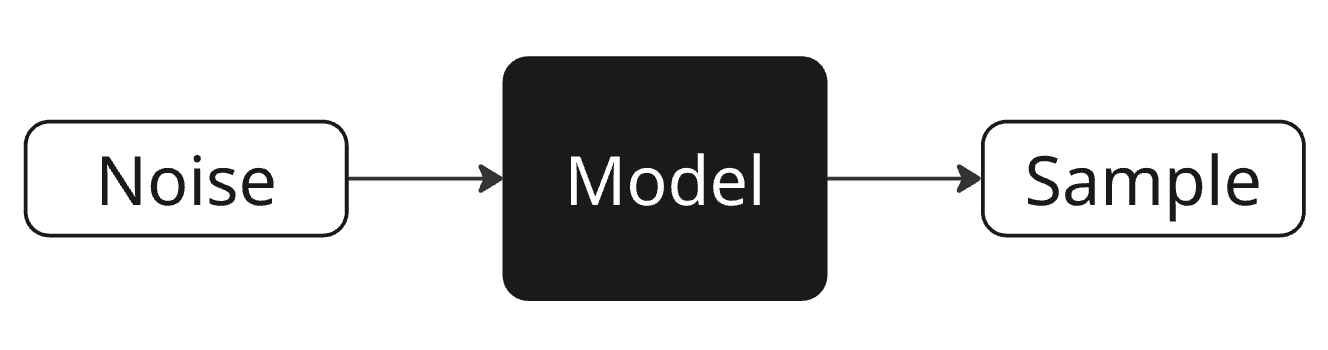
\includegraphics[width=0.95\linewidth]{figs/uncond_model}
			\end{figure}
		\end{block}
	\end{minipage}%
	\begin{minipage}{0.5\linewidth}
		\vspace{0.2cm}
		\begin{block}{Conditional model}
			\begin{figure}
				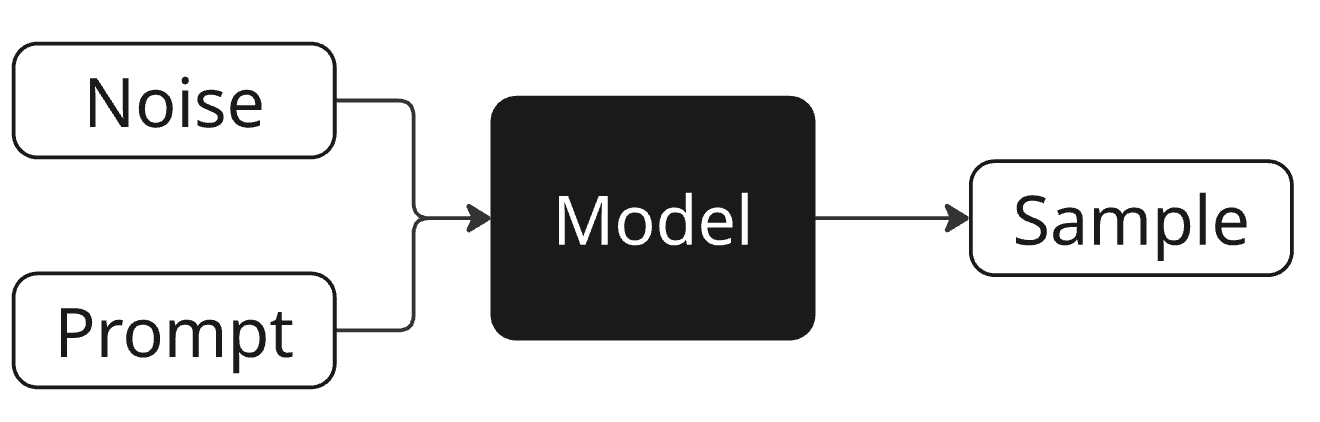
\includegraphics[width=0.95\linewidth]{figs/cond_model}
			\end{figure}
		\end{block}
	\end{minipage}
	We need the way to measure not only generated image quality, but also its relevance to the prompt.
	\begin{figure}
		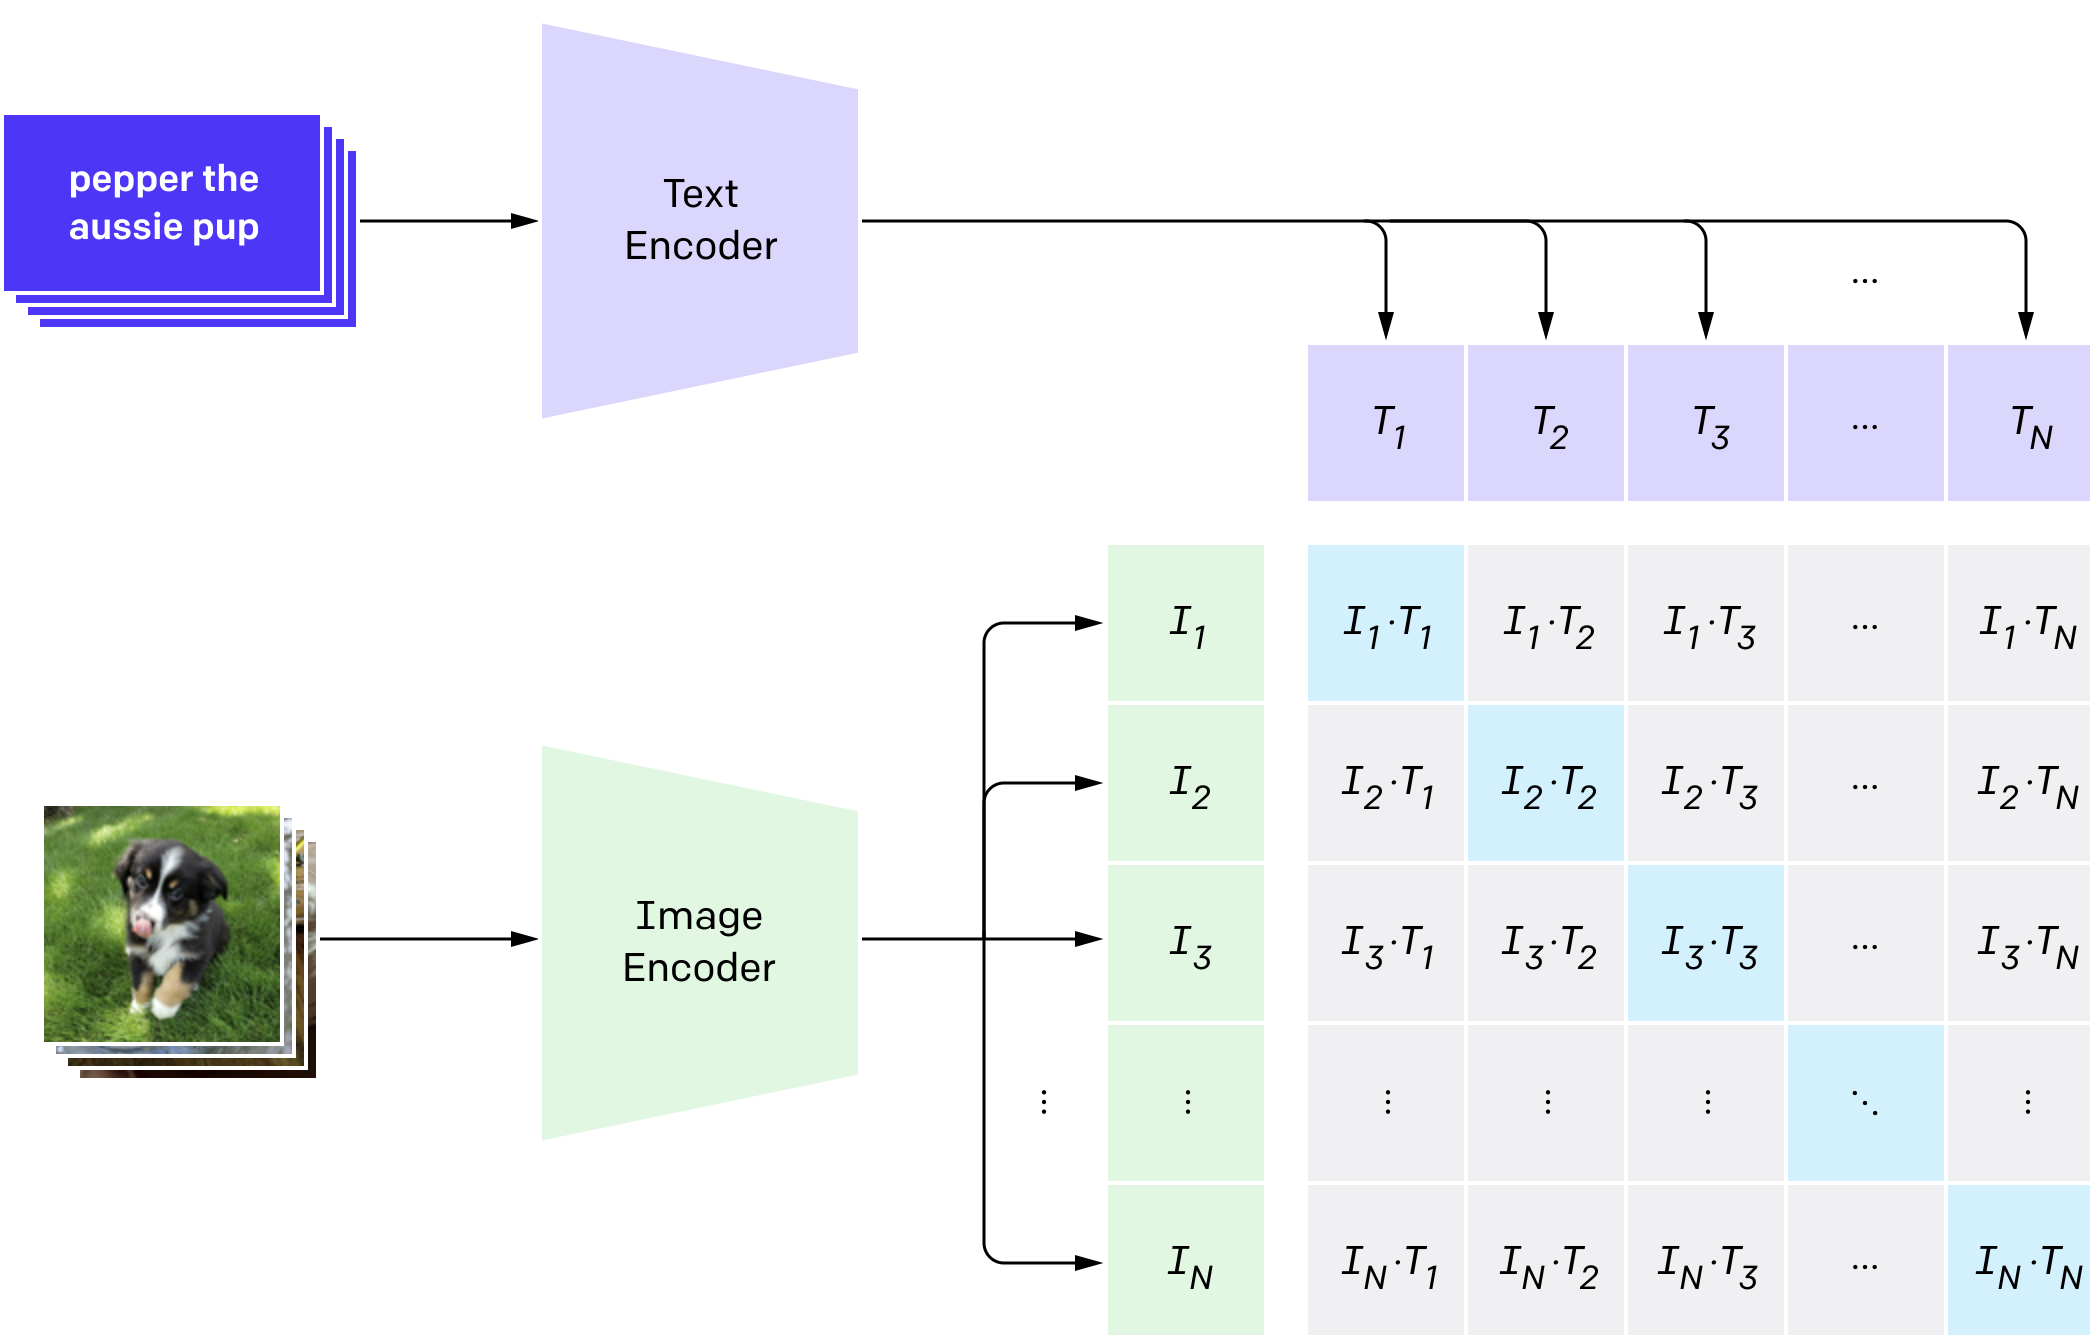
\includegraphics[width=0.6\linewidth]{figs/clip}
	\end{figure}
	\myfootnotewithlink{https://arxiv.org/pdf/2103.00020}{Radford A. et al. Learning transferable visual models from natural language supervision, 2021} 
\end{frame}
%=======
\subsection{Human evaluation}
%=======
\begin{frame}{Human Evaluation}
	\begin{itemize}
		\item There is no perfect automated metric.
		\item The best way to evaluate the generative model is to make human evaluation.
		\item It is essential to evaluate different aspects.
	\end{itemize}
	\begin{figure}
		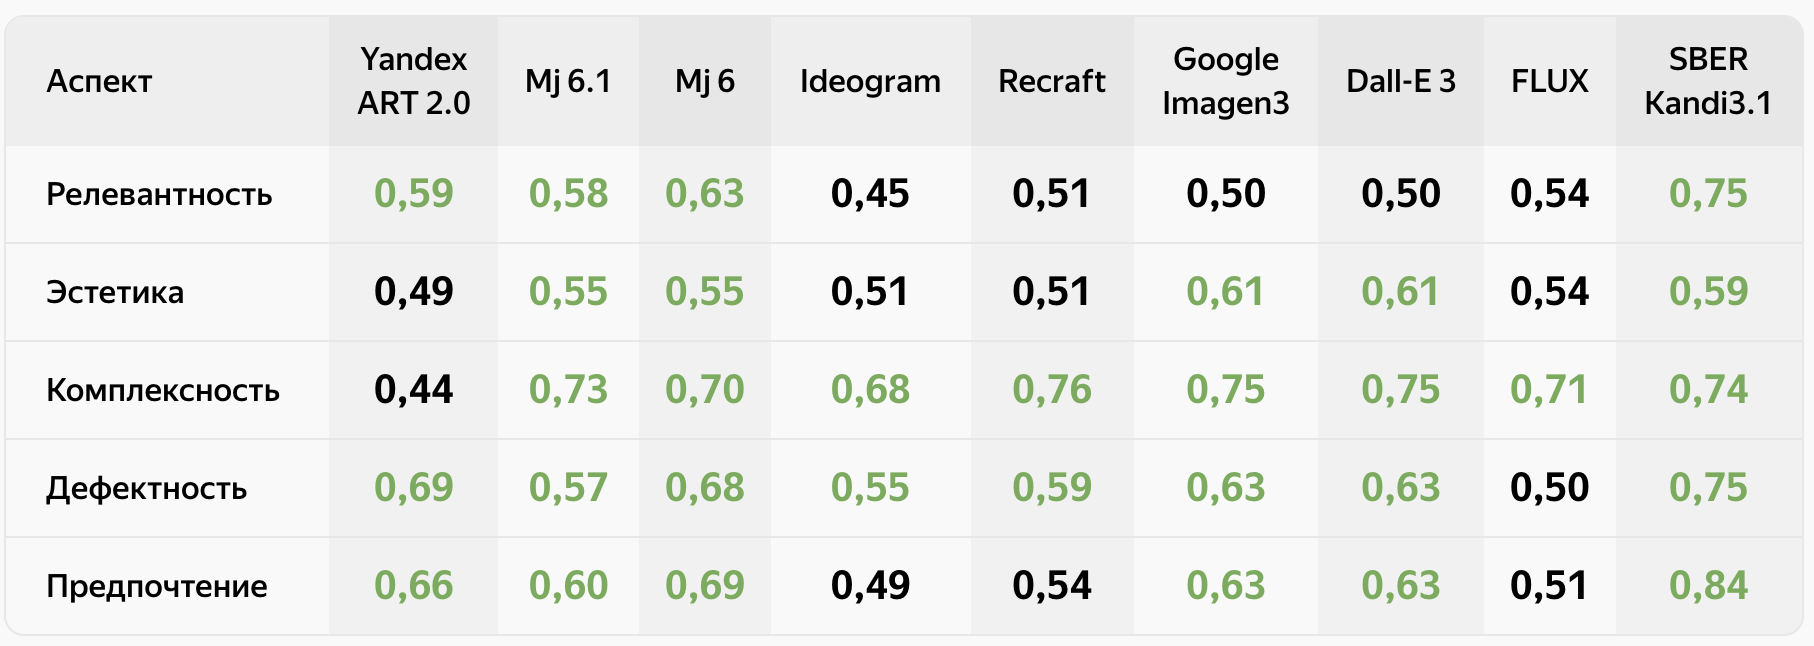
\includegraphics[width=1.0\linewidth]{figs/yaart_2.5}
	\end{figure}
	\myfootnotewithlink{https://ya.ru/ai/art}{YandexART 2.5, 2025} 
\end{frame}
%=======
\section{Langevin dynamic}
%=======
\begin{frame}{Energy-based models}
	\begin{block}{Unnormalized density}
		\vspace{-0.2cm}
		\[
			p(\bx | \btheta) = \frac{\hat{p}(\bx | \btheta)}{Z_{\btheta}}, \quad \text{where } Z_{\btheta} = \int \hat{p}(\bx | \btheta) d \bx
		\]
		\vspace{-0.3cm}
		\begin{itemize}
			\item $\hat{p}(\bx | \btheta)$ is any non-negative function. \\
			\item If we use the reparametrization $\hat{p}(\bx | \btheta) = \exp(-f_{\btheta}(\bx))$, we remove the non-negativite constraint.
		\end{itemize}
	\end{block}
	\vspace{-0.3cm}
	\begin{block}{Unnormalized density}
		The gradient of the normalized log-density equals to the gradient of the unnormalized log-density:
		\[
			\nabla_{\bx} \log p(\bx | \btheta) = \nabla_{\bx} \log \hat{p}(\bx | \btheta) - \nabla_{\bx} \log Z_{\btheta} = \nabla_{\bx} \log \hat{p}(\bx | \btheta)
		\]
	\end{block}
	\vspace{-0.3cm}
	\begin{itemize}
		\item Let assume that we already have the density (normalized or unnormalized) $p(\bx | \btheta)$.
		\item How to sample from the model?
	\end{itemize}
\end{frame}
%=======
\begin{frame}{Langevin dynamic}
	\vspace{-0.4cm}
	\begin{block}{Theorem (informal)}
		Let $\bx_0$ be a random vector. Under some mild regularity conditions samples from the following dynamics will come from $p(\bx | \btheta)$ (for small enough $\eta$ and large enough $l$)
		\vspace{-0.3cm}
		\[
			\bx_{l + 1} = \bx_l + \frac{\eta}{2} \cdot \nabla_{\bx_l} \log p(\bx_l | \btheta) + \sqrt{\eta} \cdot \bepsilon_l, \quad \bepsilon_l \sim \cN(0, \bI).
		\]
		\vspace{-0.5cm}
	\end{block}
	\begin{minipage}{0.55\linewidth}
		\begin{itemize}
			\item What do we get if $\bepsilon_l = \boldsymbol{0}$?
			\item The density $p(\bx | \btheta)$ is a \textbf{stationary} distribution for the Markov chain. 
			\item We take the gradient w.r.t. to $\bx$ (not $\btheta$).
			\item $\nabla_{\bx} \log p(\bx | \btheta)$ defines the vector field.
		\end{itemize}
	\end{minipage}%
	\begin{minipage}{0.45\linewidth}
		\begin{figure}
			\centering
			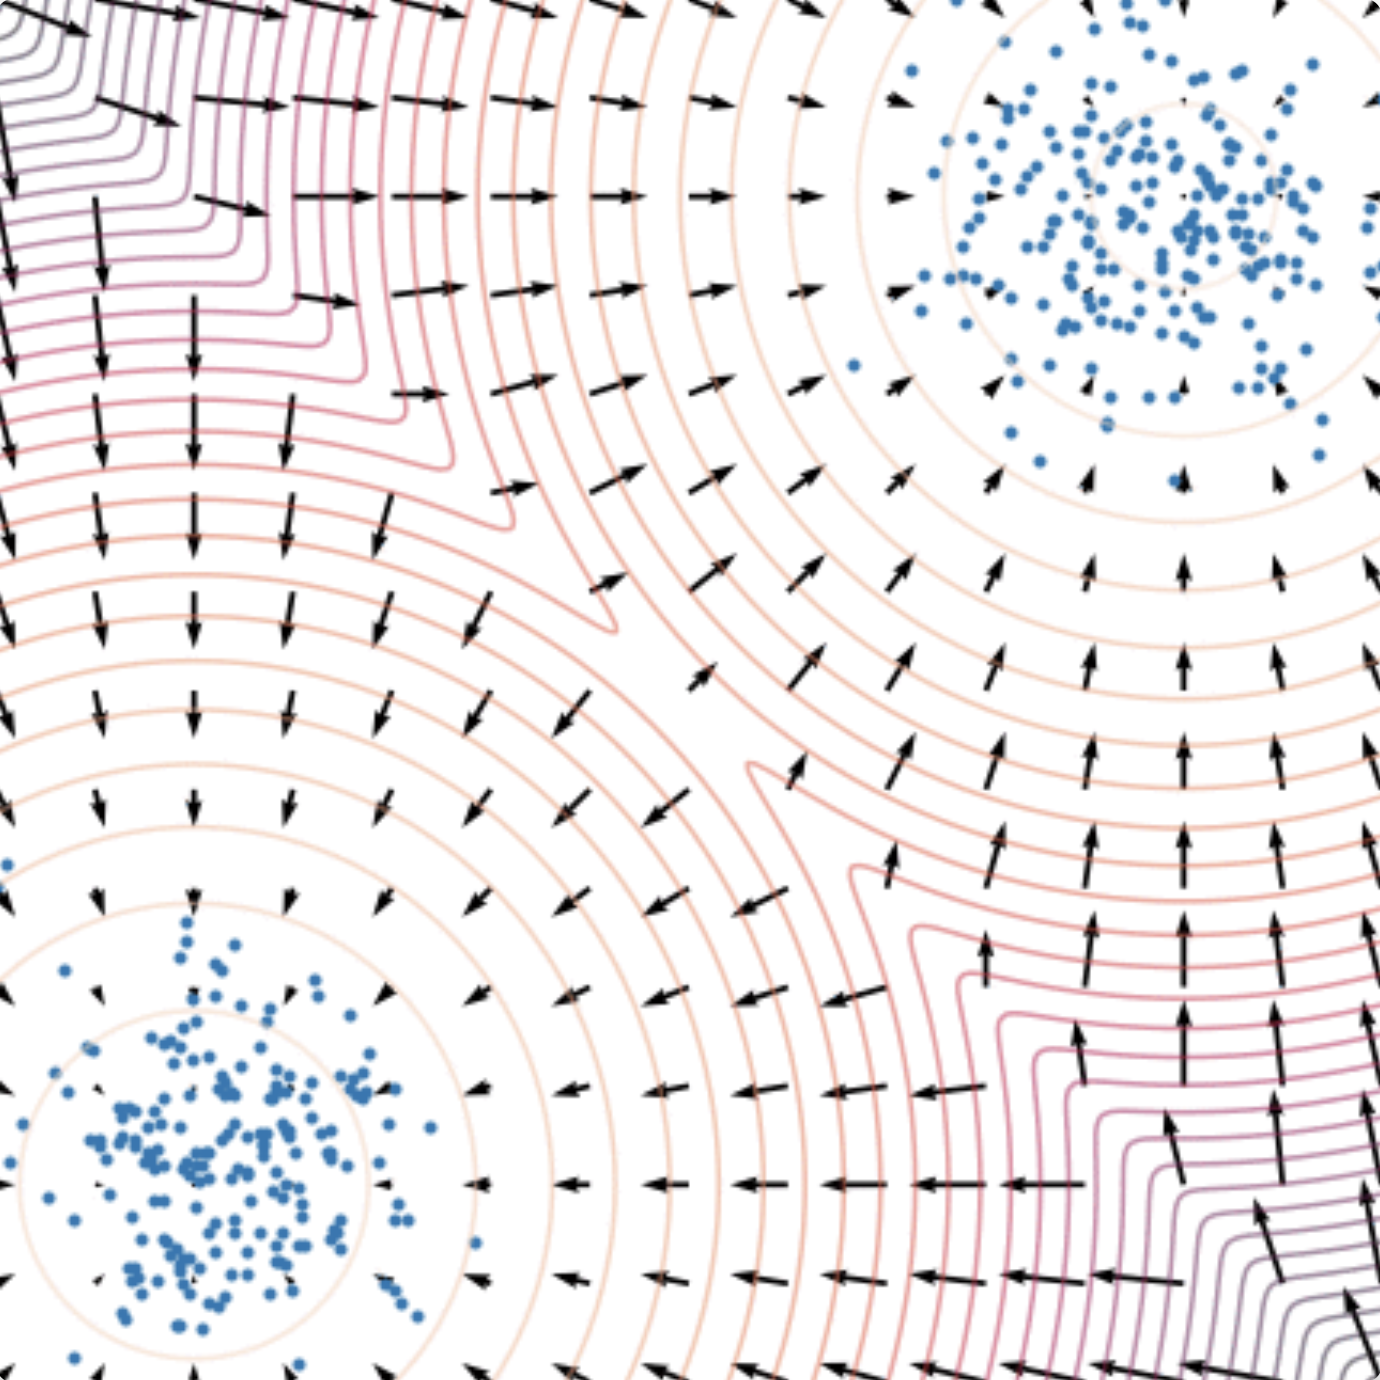
\includegraphics[width=0.9\linewidth]{figs/langevin_dynamic}
		\end{figure}
	\end{minipage}
	\myfootnotewithlink{https://yang-song.github.io/blog/2021/score/}{Song Y. Generative Modeling by Estimating Gradients of the Data Distribution, blog post, 2021} 
	\end{frame}
%=======
\section{Score matching}
%=======
\begin{frame}{Score matching}
	\begin{block}{Score function}
		\vspace{-0.3cm}
		 \[
			 \bs_{\btheta}(\bx) = \nabla_{\bx}\log p(\bx| \btheta)
		 \]
		\vspace{-0.5cm} 
	\end{block}
	\begin{block}{Langevin dynamic}
		If we find the score function $\bs_{\btheta}(\bx) = \nabla_{\bx}\log p(\bx| \btheta)$ we will be able to sample from the model using Langevin dynamic. 
		\[
			\bx_{l + 1} = \bx_l + \frac{\eta}{2} \cdot {\color{violet}\nabla_{\bx_l} \log p(\bx_l | \btheta)} + \sqrt{\eta} \cdot \bepsilon_l = \bx_l + \frac{\eta}{2} \cdot  {\color{violet}\bs_{\btheta}(\bx_l)} + \sqrt{\eta} \cdot \bepsilon_l.
		\] 
		\vspace{-0.5cm} 
	\end{block}
	\begin{block}{Fisher divergence}
		\vspace{-0.5cm}
		\begin{multline*}
			D_F(\pi, p) = \frac{1}{2}\bbE_{\pi}\bigl\| \nabla_{\bx}\log p(\bx| \btheta) - \nabla_\bx \log \pi(\bx) \bigr\|^2_2 = \\ 
			= \frac{1}{2}\bbE_{\pi}\bigl\| \bs_{\btheta}(\bx) - \nabla_\bx \log \pi(\bx) \bigr\|^2_2 \rightarrow \min_{\btheta}
		\end{multline*}
		\vspace{-0.3cm}
	\end{block}
	\myfootnotewithlink{https://yang-song.github.io/blog/2021/score/}{Song Y. Generative Modeling by Estimating Gradients of the Data Distribution, blog post, 2021}
\end{frame}
%=======
\begin{frame}{Score matching}
	\begin{block}{Fisher divergence}
		\vspace{-0.3cm}
		\[
			D_F(\pi, p) = \frac{1}{2}\bbE_{\pi}\bigl\| \bs_{\btheta}(\bx) - \nabla_\bx \log \pi(\bx) \bigr\|^2_2 \rightarrow \min_{\btheta}
		\]
		\vspace{-0.5cm}
	\end{block}
	\begin{figure}
		\centering
		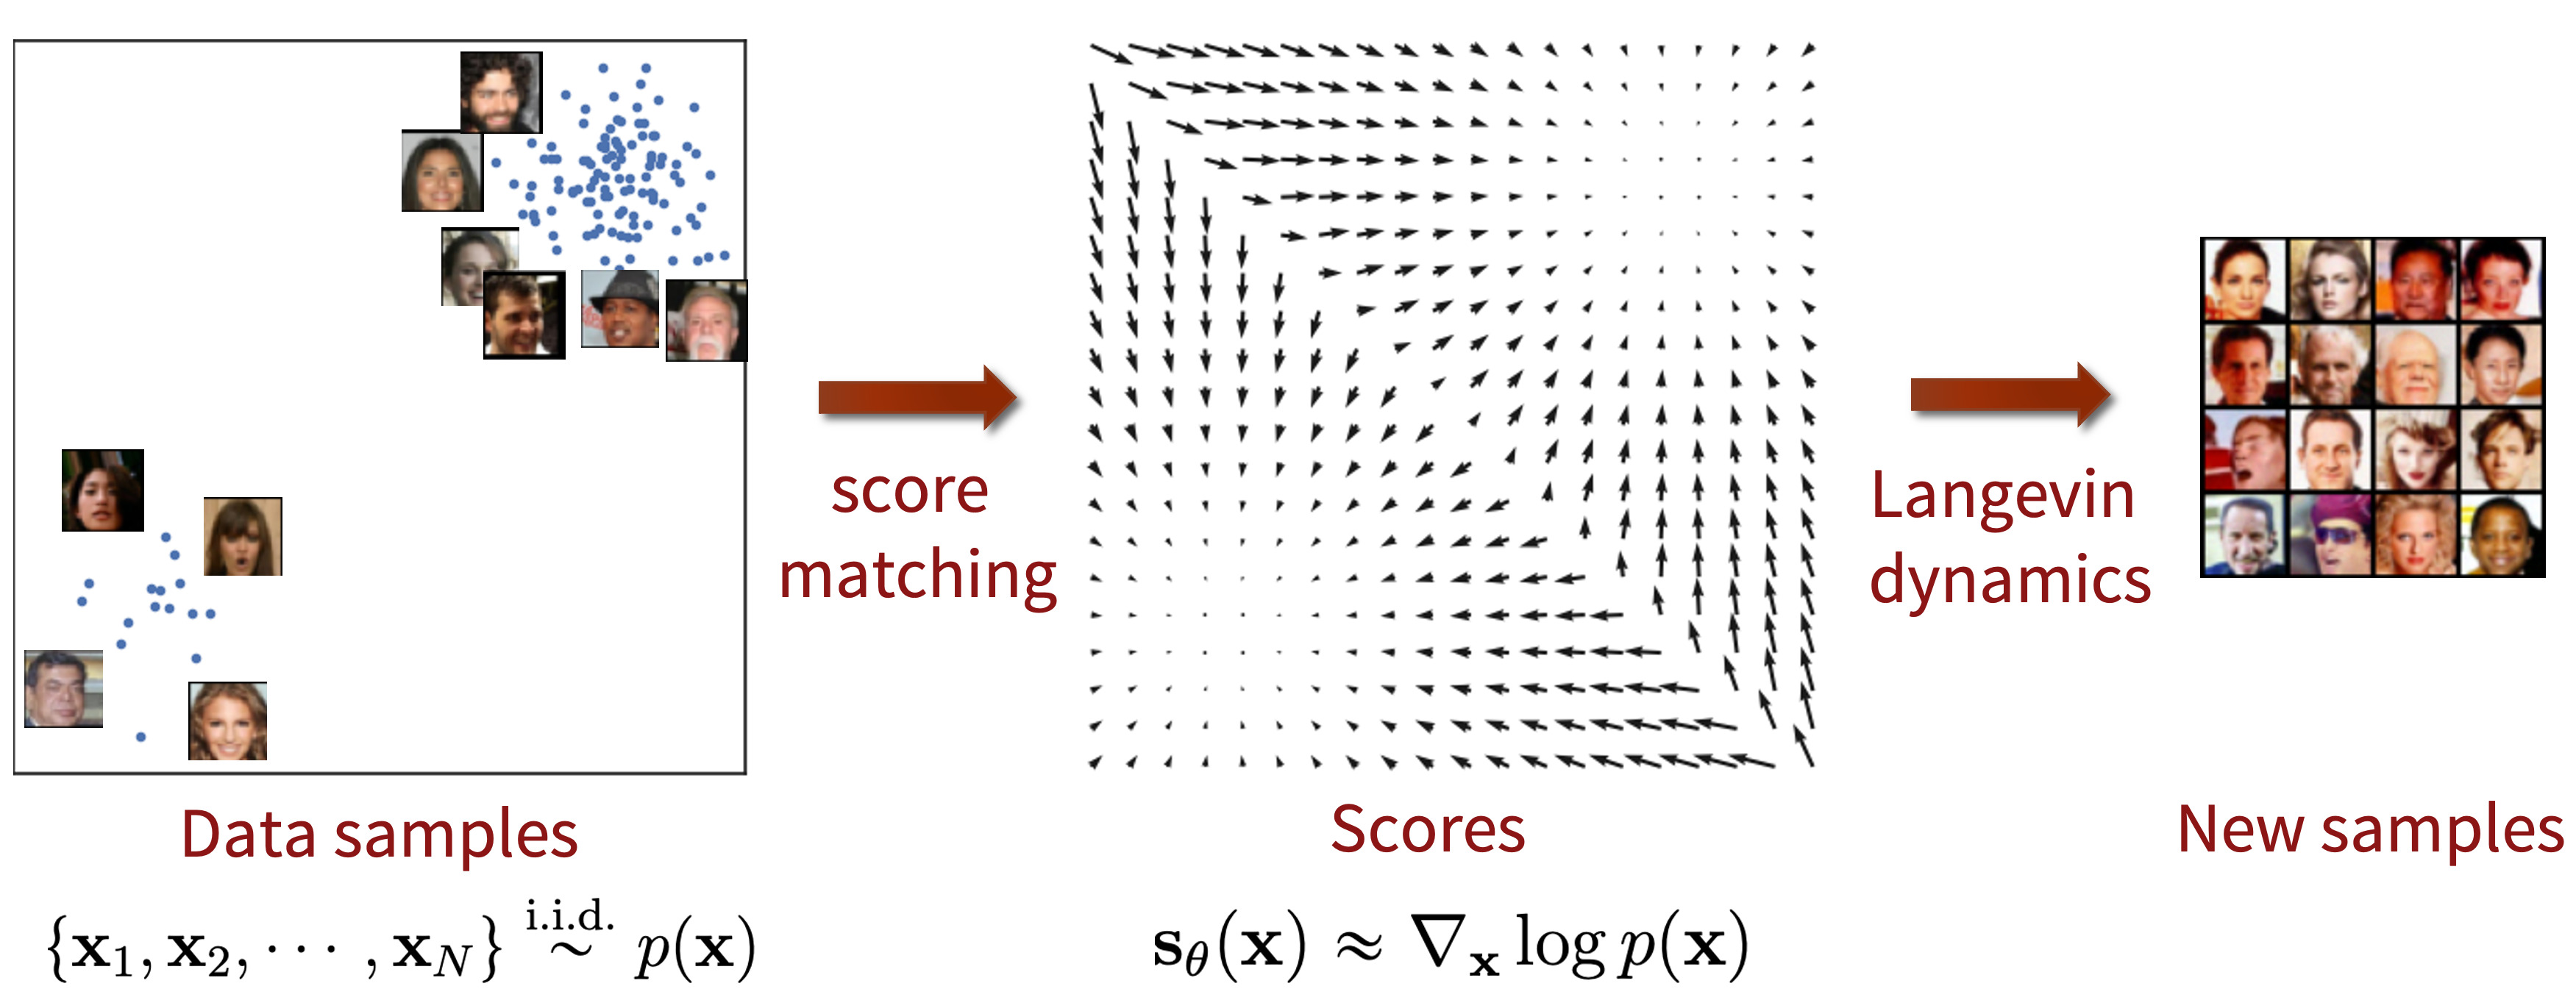
\includegraphics[width=\linewidth]{figs/smld}
	\end{figure} 
	\textbf{Problem:} We do not know $\nabla_\bx \log \pi(\bx)$.
	\myfootnotewithlink{https://yang-song.github.io/blog/2021/score/}{Song Y. Generative Modeling by Estimating Gradients of the Data Distribution, blog post, 2021}
\end{frame}
%=======
\section{Denoising score matching}
%=======
\begin{frame}{Denoising score matching}
	Let perturb original data $\bx \sim \pi(\bx)$ by random normal noise 
	\[
		\bx_{\sigma} = \bx + \sigma \cdot \bepsilon, \quad \bepsilon \sim \cN(0, \bI), \quad q(\bx_{\sigma} | \bx) = \cN(\bx, \sigma^2 \cdot \bI)
	\]
	\vspace{-0.4cm}
	\[
		q(\bx_{\sigma}) = \int q(\bx_{\sigma} | \bx) \pi(\bx) d\bx.
	\]
	\vspace{-0.5cm} 
	\begin{block}{Assumption}
		The solution of 
		\[
			\frac{1}{2} \bbE_{q(\bx_{\sigma})}\bigl\| \bs_{\btheta, \sigma}(\bx_{\sigma}) - \nabla_{\bx_{\sigma}} \log q(\bx_{\sigma}) \bigr\|^2_2 \rightarrow \min_{\btheta}
		\]
		\vspace{-0.3cm} \\
		satisfies $\bs_{\btheta, \sigma}(\bx_{\sigma}) \approx \bs_{\btheta, 0}(\bx_0) = \bs_{\btheta}(\bx)$ if $\sigma$ is small enough.
	\end{block}
	\begin{itemize}
		\item The score function of the noised data is almost the same as the score function of the original data.
		\item Score function $\bs_{\btheta, \sigma}(\bx_{\sigma})$ parametrized by $\sigma$. 
		\item \textbf{Note:} We don't know $q(\bx_{\sigma})$, just like $\pi(\bx)$.
	\end{itemize}
	\myfootnotewithlink{http://www.iro.umontreal.ca/~vincentp/Publications/smdae_techreport.pdf}{Vincent P. A Connection Between Score Matching and Denoising Autoencoders, 2010}
\end{frame}
%=======
\begin{frame}{Denoising score matching}
	\begin{block}{Theorem}
	\vspace{-0.5cm}
	\begin{multline*}
		\bbE_{q(\bx_{\sigma})}\bigl\| \bs_{\btheta, \sigma}(\bx_{\sigma}) - \nabla_{\bx_{\sigma}} \log q(\bx_{\sigma}) \bigr\|^2_2 = \\
		= \bbE_{\pi(\bx)} \bbE_{q(\bx_{\sigma} | \bx)}\bigl\| \bs_{\btheta, \sigma}(\bx_{\sigma}) - \nabla_{\bx_{\sigma}} \log q(\bx_{\sigma} | \bx) \bigr\|^2_2 + \text{const}(\btheta)
	\end{multline*}
	\vspace{-0.5cm}
	\end{block}
	\begin{block}{Gradient of the noise kernel}
		\vspace{-0.3cm}
		\[
			\bx_{\sigma} = \bx + \sigma \cdot \bepsilon, \quad q(\bx_{\sigma} | \bx) = \cN(\bx, \sigma^2 \cdot \bI)
		\]
		\vspace{-0.3cm}
		\[
			\nabla_{\bx_{\sigma}} \log q(\bx_{\sigma} | \bx) = - \frac{\bx_{\sigma} - \bx}{\sigma^2}  = - \frac{\bepsilon}{\sigma}
		\]
		\vspace{-0.5cm}
	\end{block}
	\begin{itemize}
		\item The RHS does not need to compute $\nabla_{\bx_{\sigma}} \log q(\bx_{\sigma})$ and even $\nabla_{\bx_{\sigma}} \log \pi(\bx_{\sigma})$.
		\item $\bs_{\btheta, \sigma}(\bx_{\sigma})$ tries to \textbf{denoise} the noised samples $\bx_{\sigma}$. 
	\end{itemize}
	\myfootnotewithlink{http://www.iro.umontreal.ca/~vincentp/Publications/smdae_techreport.pdf}{Vincent P. A Connection Between Score Matching and Denoising Autoencoders, 2010}
\end{frame}
%=======
\begin{frame}{Denoising score matching}
	Initial objective:
	\vspace{-0.2cm}
	\[
		\bbE_{\pi(\bx)}\bigl\| \bs_{\btheta}(\bx) - \nabla_\bx \log \pi(\bx) \bigr\|^2_2 \rightarrow \min_{\btheta}
	\]
	\vspace{-0.5cm} \\
	Noised objective:
	\vspace{-0.2cm}
	\[
		\bbE_{q(\bx_{\sigma})}\bigl\| \bs_{\btheta, \sigma}(\bx_\sigma) - \nabla_\bx \log q(\bx_{\sigma}) \bigr\|^2_2 \rightarrow \min_{\btheta}
	\]
	\vspace{-0.5cm} \\
	This is equivalent to denoising task
	\vspace{-0.2cm}
	\[
		\bbE_{\pi(\bx)} \bbE_{q(\bx_{\sigma} | \bx)}\bigl\| \bs_{\btheta, \sigma}(\bx_{\sigma}) - \nabla_{\bx_{\sigma}} \log q(\bx_{\sigma} | \bx) \bigr\|^2_2 \rightarrow \min_{\btheta}
	\]
	\vspace{-0.3cm}
	\[
		\bbE_{\pi(\bx)} \bbE_{\cN(0, \bI)}\left\| \bs_{\btheta, \sigma}(\bx + \sigma \cdot \bepsilon) + \frac{\bepsilon}{\sigma} \right\|^2_2 \rightarrow \min_{\btheta}
	\]
	\vspace{-0.5cm}
	\begin{block}{Langevin dynamic}
		\vspace{-0.3cm}
		\[
			\bx_{l + 1} = \bx_l + \frac{\eta}{2} \cdot \bs_{\btheta, \sigma}(\bx_l) + \sqrt{\eta} \cdot \bepsilon_l, \quad \bepsilon_l \sim \cN(0, \bI).
		\]
		\vspace{-0.7cm}
	\end{block}
	\myfootnotewithlink{https://yang-song.github.io/blog/2021/score/}{Song Y. Generative Modeling by Estimating Gradients of the Data Distribution, blog post, 2021}
\end{frame}
%=======
\begin{frame}{Summary}
	\begin{itemize}
		\item Frechet Inception Distance is the most popular metric for the implicit models evaluation. 
		\vfill
		\item Precision-recall allow to select model that compromises the sample quality and the sample diversity.	
		\vfill 
		\item CLIP score is frequently used to measure text-to-image relevance.
		\vfill
		\item The best way to measure the generated image quality is to make human evaluation.
		\vfill
		\item Langevin dynamics allows to sample from the generative model using the gradient of the log-likelihood.	
		\vfill
		\item Score matching proposes to minimize the Fisher divergence to get the score function.
		\vfill 
		\item Denoising score matching minimizes the Fisher divergence on noisy samples. It allows to estimate the Fisher divergence using samples.
	\end{itemize}
\end{frame}
\end{document} 